\documentclass{article}
\usepackage{graphicx}
\usepackage[utf8]{inputenc}
\usepackage{amsmath}
\usepackage{amssymb}
\usepackage{graphicx}
\usepackage{epstopdf}
\usepackage{inputenc}
\usepackage{latexsym}
\usepackage{setspace}
\usepackage{caption}
\usepackage{authblk}
\setlength\parindent{24pt}


\begin{document}

\title{Programming and data analysis in Labwindows}
\author{Loïc James McKeever}
\affil{Mackenzie Levangie}

\maketitle

\section{Introduction}


 The goal of this lab is to analyze a given set of data.  Specifically the analysis will consist of plotting the data, subtracting a baseline, normalizing the data and finding the centroid of the largest peak.  This will be done using Labwindows and program will be written in C.  The data given has no known units or meaning so we will use x and y.  We subtracted a baseline of 2.5 y and found the centroid to be at 63 x.

\section{Materials and Methods}

The code used had several different functions and was designed to be as general as possible.  The UI panel allowed the user to select any file they wanted.  Once selected the code counted the number of lines of data and converted the data into a single array.  This is done by using a for-loop to look at each character, if the character is a new line character ('\textbackslash n') then it adds one to a counter until it reaches EOF(end of file).  The file is then converted to an array that is twice the size of the number of lines since there are two data points per line.  The only drawback is that the code assumes that the data is in only two columns.
\\
Once the file is selected the user can display the file which divides the array into two arrays, X and Y, and plots them on the UI panel.  This is done using two for loops.  One loop moves every other data point into the X array starting at the first point while the other loop moves every other data point into the Y array starting at the second data point.  This is done because when the file is first converted into an array each data point is listed one after the other by line.
\\
Further analysis can also be done including setting a baseline value on the UI panel and then subtracting that baseline from the data points.  This is done using a simple for-loop and an input control.  The data can be normalized and the normalization factor will be displayed on the UI panel.  This is done by doing a Riemann sum and then dividing each data point by that area(the normalization factor).  Finally the position of the centroid can be determined and displayed.  This is done by doing a Riemann sum to get the total area of the curve and then doing it again but at each X data point subsequently until half the total area is reached using an if statement.  That position is saved and a line is displayed on the graph for visual assessment.  Lastly the analyzed data can be saved to a text file from the UI panel.  The data was then plotted again using a simple scatter plot in Excel.



\section{Results}

The first step was to simply read the data, convert the data into an array and then plot the data without modifying it.  See fig. 1.

\begin{figure}[h!]
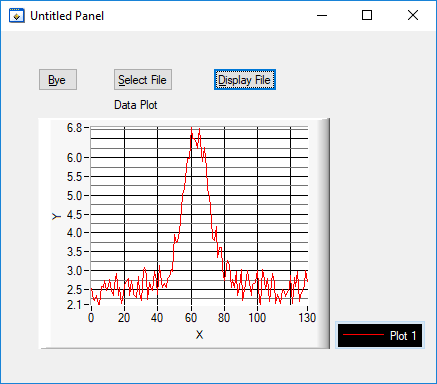
\includegraphics{Lab1_1.png}
\caption{This figure shows the data plotted as it was received without normalization or baseline subtraction.  We do notice however that most of the data is around 2.5 Y aside from a relatively large peak at 60 X.}
\end{figure}

The next step is to implement the various analysis tools;  baseline subtraction, normalization and centroid calculation.  Once those modification have been made to the data we can plot it again.  See fig. 2.
\\

\begin{figure}[h!]
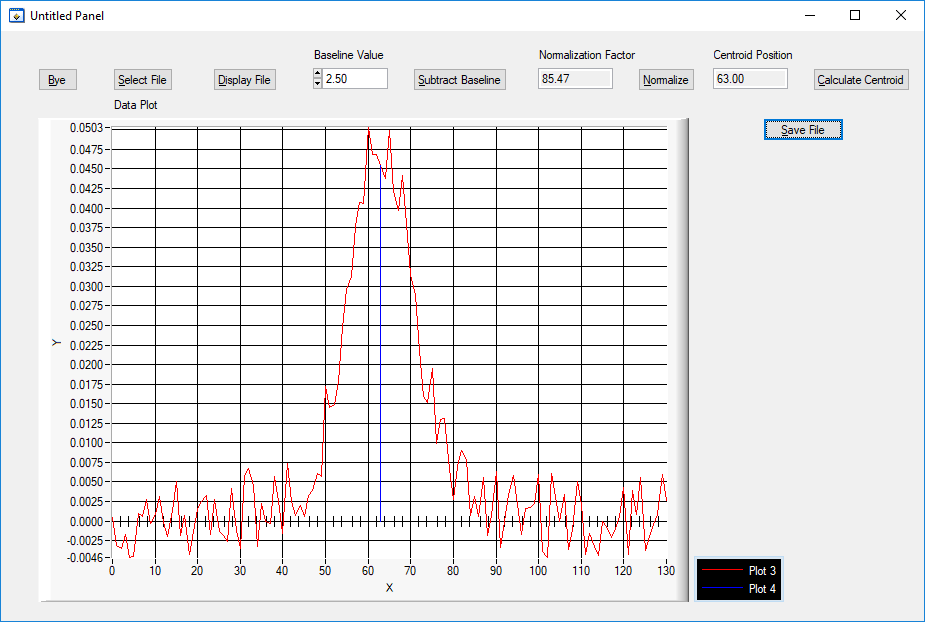
\includegraphics[scale=.475]{Lab1_2.png}
\caption{This figure shows the data plotted after a baseline of 2.5 Y was subtracted and the data was normalized.  We can also note that the normalization factor is displayed(85.47 X.Y) as well as the X position of the centroid(63 X). We can visually evaluate that the centroid position is accurate.}
\end{figure}

Finally the modified data can be saved and used in other programs such as Excel.  See fig. 3.

\begin{figure}[h!]
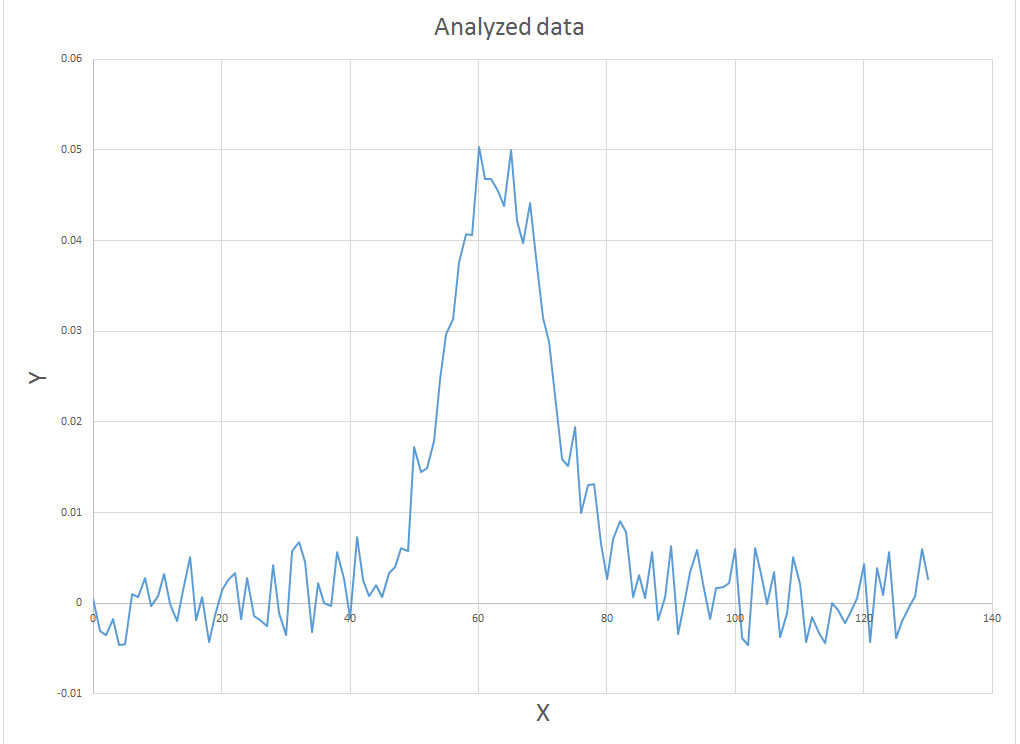
\includegraphics[scale=.95]{Lab1_Plot.jpg}
\caption{This figure shows the modified data plotted in Excel.  This allows easier visualization as well as easier graph customization.}
\end{figure}

\newpage

\section{Discussion}
For this particular lab this section won't be a substantial as it usually since there was no known context for the data given. 
\\
We can note however that the program written for this lab could potentially used in other labs, with perhaps a few modifications.  If we regard the data as a test of the performance of the code we can discuss the viability of using the code in the future.  The code can be used for any kind of data set with two distinct columns.  It could potentially be used for data sets with more than two columns with relatively simple modifications.  These modifications would mostly need to be done when the code divides the data set up by column and at the end when it saves the modified data to a file.  The analysis sections might also need some tweaking for higher dimensions but again that should be relatively straightforward.  

\section{Conclusion}

In conclusion our code was able to take data from any file of the users choosing and allowed the users to perform a variety of analysis techniques.  This included plotting, baseline subtraction(in our case a baseline of 2.5 Y), normalization(in our case a normalization factor of 85.47 X.Y) and centroid localization(in our case at 63 X).  This code could also be used with other data sets given perhaps a few minor modifications.

\section{Appendix}

See code attached.


\end{document}
